\section{What is SOLID?} % (fold)
\label{sec:what_is_solid_}

% section what_is_solid_ (end)

\section{S - Single Responsibility Principle } % (fold)
\label{sec:s}

\begin{frame}
	\say{\textit{Every class should have responsibility over a single part of the functionality
  provided by the software, and that responsibility should be entirely encapsulated by the
  class.}}, \\DeMarco, Tom
\end{frame}

\begin{frame}
  \begin{figure}[p]
        \centering
        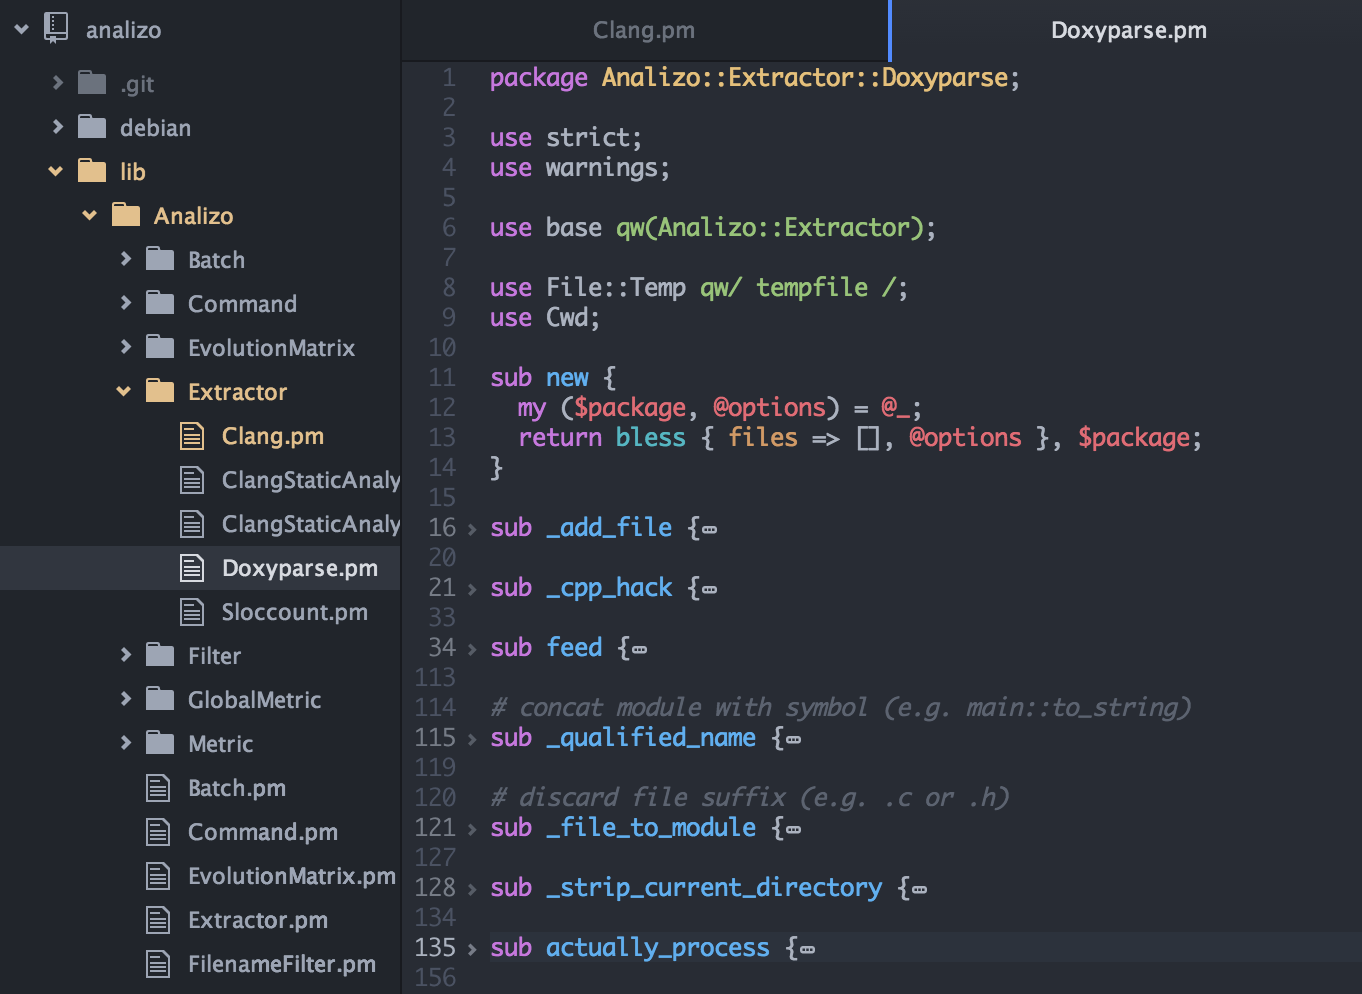
\includegraphics[width=0.8\textwidth]{doxyparse_pattern.png}
        \label{fig:Pattern}
    \end{figure}
\end{frame}

\begin{frame}
  \begin{figure}[p]
        \centering
        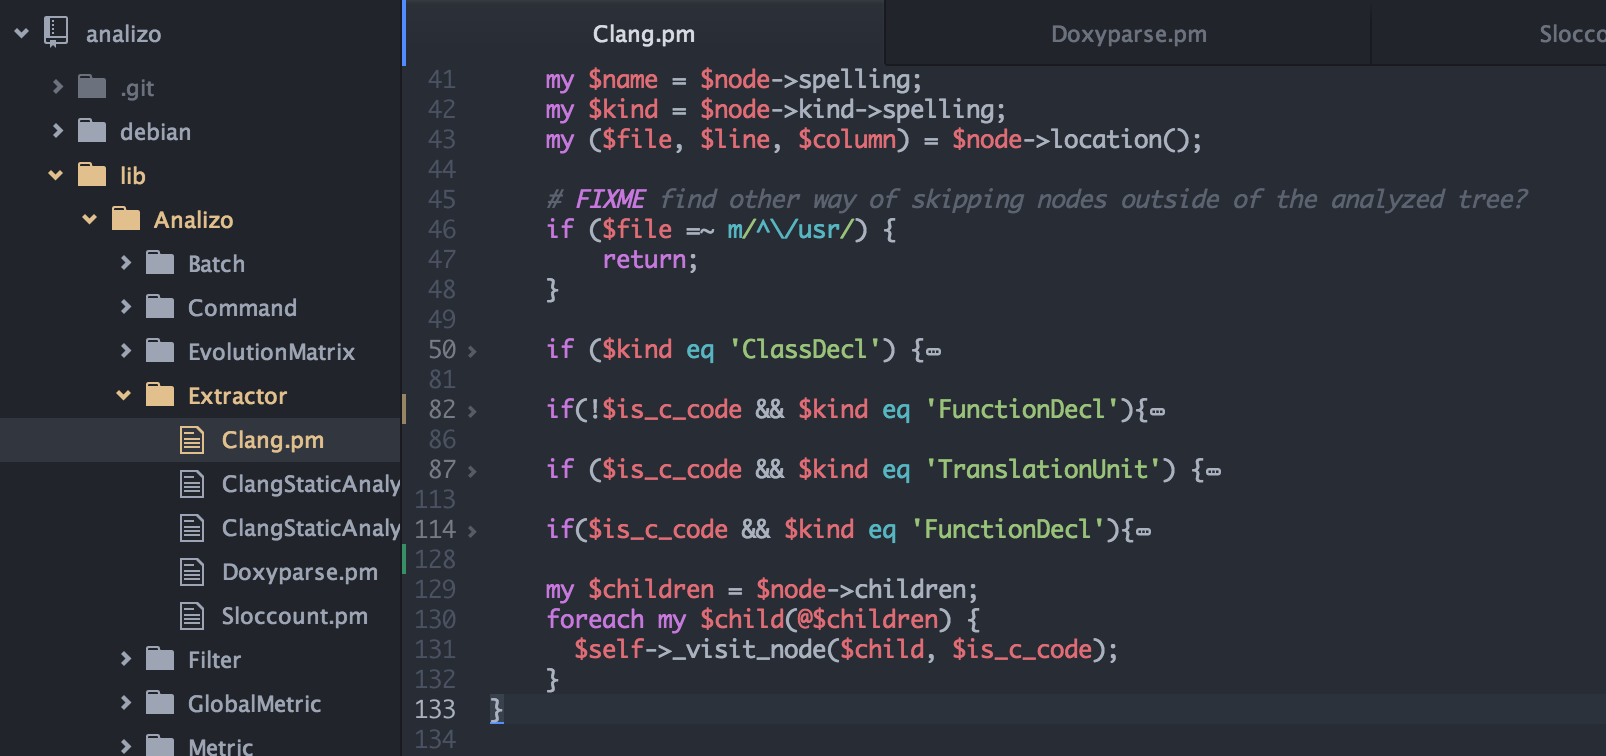
\includegraphics[width=0.8\textwidth]{clang_antipattern.png}
        \label{fig:antiPattern}
    \end{figure}
\end{frame}

% section s (end)


\section{O - Open/closed principle} % (fold)
\label{sec:o}

\begin{frame}
	\say{\textit{Software entities should be open for extension, but closed for modification.}}, \\Meyer, Bertrand
\end{frame}

\begin{frame}


\begin{Parallel}[v]{5cm}{5cm}
    \ParallelLText%
    {
    	\textbf{Bertrand Meyer, 1988}

    	The idea was that once completed, the implementation of a class could only be modified to correct errors.
    }
    \ParallelRText%
    {
    	\textbf{1990s}

    	The implementations can be changed and multiple implementations could be created and polymorphically substituted for each other.
	}
\end{Parallel}

\end{frame}

\subsection{Use in Analizo} % (fold)
\label{sub:use_in_analizo}
\begin{frame}

\begin{figure}[h!]
  % \caption{The Extractor inherited.}
  \centering
    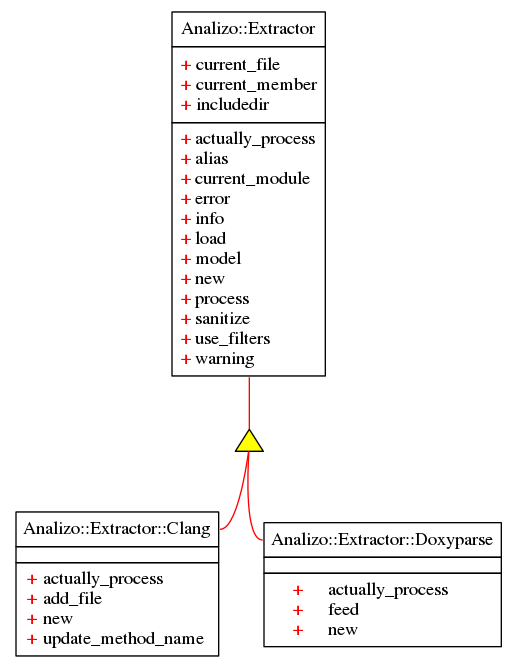
\includegraphics[width=0.5\textwidth]{conteudo/Extractor}
    \caption{Extractor inherited}
\end{figure}
    
\end{frame}
% subsection use_in_analizo (end)


% section o (end)

\section{L} % (fold)
\label{sec:l}

% section l (end)

\section{I - Interface segregation principle} % (fold)
\label{sec:i}
\begin{frame}
	\say {\textit{Client should not be forced to depend on methods it does not use}},\\Martin, Robert(2002)
\end{frame}
\begin{frame}
\begin{figure}
        \centering
        \begin{minipage}{.5\textwidth}
            \centering
            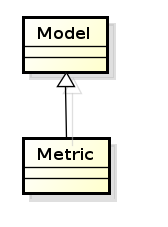
\includegraphics[width=.4\linewidth]{ipossivelerro2.png}
            \caption{Model was a abstraction class}
        \end{minipage}%
        \begin{minipage}{.5\textwidth}
            \centering
            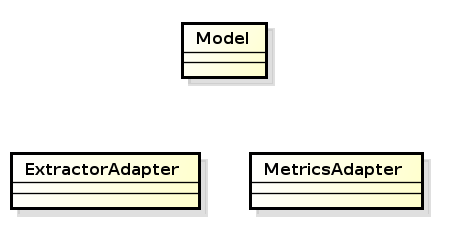
\includegraphics[width=.4\linewidth]{improvement2.png}
            \caption{Possible application of ISP}
        \end{minipage}
    \end{figure}
\end{frame}
% section i (end)

\section{D - Dependency Inversion Principle} % (fold)
\label{sec:d}

\begin{frame}
    \say{\textit{Depend upon Abstractions. Do not depend upon concretions.}}, \\Martin, Robert C.
\end{frame}

\begin{frame}
    
\begin{Parallel}[v]{5cm}{5cm}
    \textbf{Principles:}
    \ParallelLText%
    {

        High-level modules should not depend on low-level modules. Both should depend on abstractions.
    }
    \ParallelRText%
    {

        Abstractions should not depend on details. Details should depend on abstractions.
    }
\end{Parallel}  

\end{frame}
\begin{frame}

\begin{figure}[!htb]
    \centering
    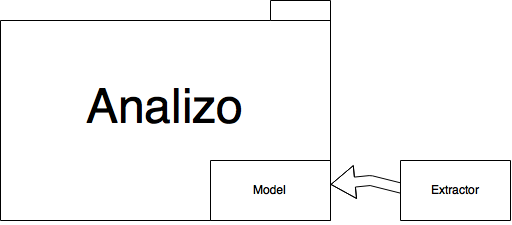
\includegraphics[scale=0.5]{SOLID-D}
    \caption{Analizo - Dependency Inversion Principle}
\end{figure}
\end{frame}

% section d (end)
\section{SOLID for our code} % (fold)
\label{sec:our_code}

\begin{frame}

Using SOLID for points of improvement in our code, wih priority to:
\begin{itemize} 
\setlength{\leftmargini}{2.5em}
\item     Single-responsiblity principle
\item     Open-closed principle 
\item     Dependency Inversion Principle
\end{itemize}
\end{frame}

\begin{frame}
\begin{figure}[!htb]
\centering
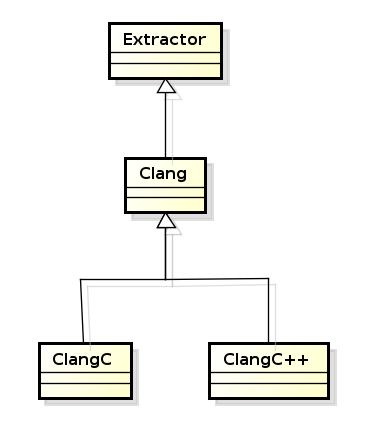
\includegraphics[scale=0.3]{SOLID_ANALIZO}
\caption{Analizo - Refactoring Clang Extractor}
\end{figure}
\end{frame}
